% Provenance (never printed): see sources/outline_sources.md (Year 1: the wind-driven
% circulation, gyres, Ekman transport and upwelling, western boundary currents, the
% meridional overturning circulation and the water masses). Exercise and problem values in
% the Book 3 scratch calculator calc/ch29.py; figures from figdata/bachelor-1/
% ekman_hodograph.py (Ekman's solution with Ekman's constants) and stommel_gyre.py
% (Stommel's 1948 model, exercise parameters), the world map from figdata/shared/geo.py.
% Physics owns the Coriolis force (recalled). Book 1 (g8) gave the surface currents and
% the gyres in words, Book 2 (g10) upwelling: re-founded here with the Ekman balance.
% Ch. 26 owns the T-S diagram and the water masses, ch. 28 the Coriolis parameter, the
% geostrophic wind and the mean meridional streamfunction. The Sverdrup balance, the
% vorticity argument and the derivation of the Ekman spiral are the Year 3 volume's; ENSO
% the Year 2 volume's.
\chapter{دوران المحيط}\label{ch:b1:ocean-circulation}

في عام 1992، أثناء عاصفة في شمال المحيط الهادئ، انزلقت حاوية عن سفينة تبحر من هونغ كونغ إلى الولايات المتحدة. انفتحت وأطلقت نحو \num{29000} بطّة مطاطية وألعابًا أخرى للاستحمام، طفت بعيدًا وسافرت في كل اتجاه؛ وساعدت الأماكن التي وُجد فيها بعضها لاحقًا العلماء على فهم التيّارات التي حملتها. تتبع الألعاب الطافية ماء السطح، وماء سطح المحيطات لا يتجوّل عشوائيًّا: فهو يدور في دوّامات تغطّي الحوض كله، ويندفع شمالًا في تيّارات ضيّقة على طول السواحل الغربية للمحيطات، ويصعد أو يهبط في أماكن قليلة مختارة. يشرح هذا الفصل كيف تحرّك الريح الطبقة العليا من المحيط، ولماذا يتحرّك الماء عموديًّا على الريح التي تدفعه، ولماذا تلتصق أقوى التيّارات بالجانب الغربي للمحيطات، وكيف يحمل انقلاب بطيء الماء إلى الأعماق ثم يعيده.
% ledger: noaa:floatees

\begin{omfigure}
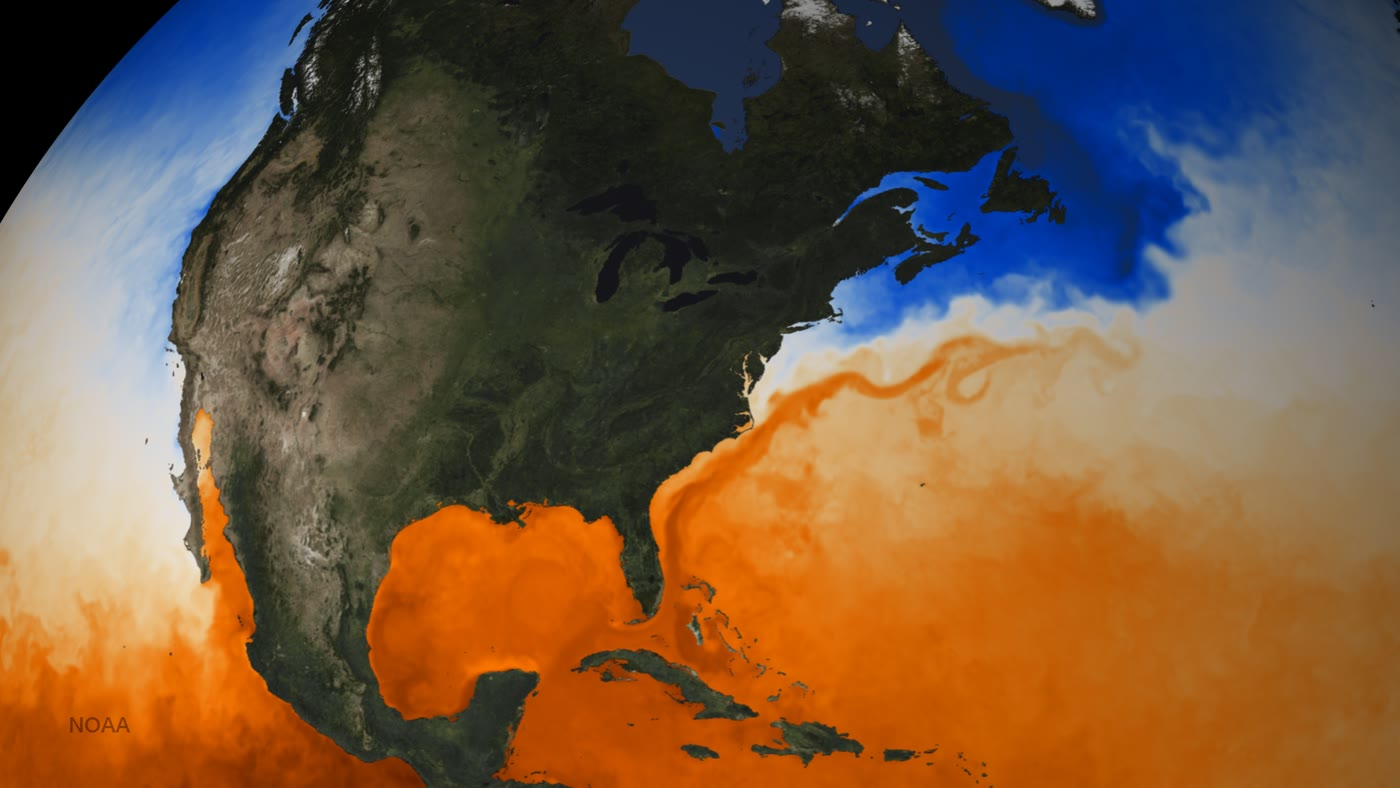
\includegraphics[width=0.85\linewidth]{images/book3/b1-gulf-stream-sst.jpg}

{\small درجة حرارة سطح البحر حول أمريكا الشمالية في أوائل يونيو 2016، من بيانات الأقمار الصناعية (الماء الدافئ باللون البرتقالي، والبارد بالأزرق). يخرج تيّار الخليج من ساحل الولايات المتحدة شريطًا دافئًا متعرّجًا، ويعبر الأطلسي نحو أوروبا؛ وعند \omterm{def:b1:spherical-astronomy:geographic}{خطوط العرض} نفسها يكون الماء قبالة ساحل المحيط الهادئ أبرد كثيرًا منه قبالة ساحل الأطلسي. (NOAA, NESDIS, ملك عام، عبر Wikimedia Commons.)}
\label{fig:b1:ocean-circulation:sst}
\end{omfigure}
% ledger: commons:gulf-stream-sst, noaa:gulf-stream-heat

\begin{recall}
تعطي كتب الفيزياء قوة كوريوليس. كتب \cref{ch:b1:atmospheric-circulation} جزأها الأفقي بالشكل $-f\,\vec k\times\vec v$، مع \omterm{def:b1:atmospheric-circulation:coriolis-parameter}{معامل كوريوليس} $f = 2\Omega\sin\varphi$ ($\Omega = \qty{7.292e-5}{rad.s^{-1}}$)، ووجد \omterm{def:b1:atmospheric-circulation:winds}{الرياح التجارية}، وهي شرقيّات بين خطّ الاستواء ونحو \ang{30}، \omterm{def:b1:atmospheric-circulation:winds}{والرياح الغربية} بعدها؛ وعرّف أيضًا \omterm{def:b1:atmospheric-circulation:streamfunction}{دالّة التيّار الميريدية المتوسطة} لدورة انقلابية. و\Cref{ch:b1:fluid-envelopes-structure} أعطى \omterm{def:b1:fluid-envelopes-structure:ocean-layers}{الطبقة المختلطة} \omterm{def:b1:fluid-envelopes-structure:ocean-layers}{والترموكلاين}، وكثافة ماء البحر، \omterm{def:b1:fluid-envelopes-structure:ts-diagram}{ومخطّط T–S} وكتل الماء في جنوب الأطلسي، و\cref{ch:b1:radiation-heat-transport} نقل الحرارة نحو القطبين الذي تتقاسمه الغلاف الجوي والمحيط. ووصف الكتاب~1 التيّارات السطحية والدوّامات الكبرى؛ ووصف الكتاب~2 صعود الماء البارد على بعض السواحل.
% ledger: earth:Trot, nos:gyres
\end{recall}

\section{الريح والتيّارات السطحية}\label{sec:b1:ocean-circulation:wind}

تحرّك الريح البحر بفركه عليه. وتنتشر قوّتها على السطح، وتُقاس، كالضغط، لكل وحدة مساحة.

\begin{definition}[إجهاد الريح]\label{def:b1:ocean-circulation:wind-stress}
\emph{إجهاد الريح}\index{إجهاد الريح} $\vec T$ هو القوة الأفقية لكل وحدة مساحة التي تؤثّر بها الريح على سطح البحر، بالباسكال. وهو نقل نحو الأسفل لزخم الهواء الأفقي إلى المحيط، ويشير تقريبًا على طول الريح. ويُعطى مقداره بالصيغة الجمعية
\[
  T = \rho_a C_D U_{10}^2,
\]
حيث $\rho_a = \qty{1.3}{kg.m^{-3}}$ كثافة الهواء، و$U_{10}$ سرعة الريح على ارتفاع \qty{10}{m} فوق البحر، و$C_D$ معامل سحب بلا بُعد.
\end{definition}
% ledger: stewart:wind-stress

يُقاس معامل السحب بأجهزة سريعة تسجّل التقلّبات المضطربة للريح على بضعة أمتار فوق الأمواج. وبالنسبة إلى هواء محايد الاستقرار، تعطي قياسات Yelland and Taylor
\[
  1000\,C_D = 0.29 + \frac{3.1}{U_{10}} + \frac{7.7}{U_{10}^2}
  \quad (\qtyrange{3}{6}{m/s}),
  \qquad
  1000\,C_D = 0.60 + 0.071\,U_{10}
  \quad (\qtyrange{6}{26}{m/s}),
\]
مع $U_{10}$ بالأمتار في الثانية. ريح قدرها \qty{10}{m/s} لها $C_D =
\num{1.31e-3}$، وتؤثّر بقوة $T = 1.3 \times \num{1.31e-3} \times 100 =
\qty{0.170}{Pa}$؛ وريح قدرها \qty{5}{m/s} تعطي \qty{0.040}{Pa}؛ وعاصفة قدرها \qty{20}{m/s} تعطي \qty{1.05}{Pa}. ومضاعفة الريح من 10 إلى \qty{20}{m/s} تضرب الإجهاد في $6.2$، لا في $4$: فالبحار الأخشن تمسك الريح أشدّ. وهذه الإجهادات ضئيلة، جزء من مليون من الضغط الجوي، لكنها تؤثّر دون توقّف في المحيط كله.
% ledger: stewart:drag-coefficient (computed in figdata/bachelor-1/ekman_hodograph.py and calc/ch29.py)

يتبع نمط الإجهاد أنماط الرياح. بين \omterm{def:b1:atmospheric-circulation:winds}{الرياح التجارية} في المدارات، التي تهبّ نحو الغرب، \omterm{def:b1:atmospheric-circulation:winds}{والرياح الغربية} في \omterm{def:b1:spherical-astronomy:geographic}{خطوط العرض} الوسطى، التي تهبّ نحو الشرق، يُدار الماء السطحي لكل حوض محيطي.

\begin{definition}[الدوّامة؛ الدوّامات شبه المدارية وشبه القطبية]\label{def:b1:ocean-circulation:gyre}
\emph{الدوّامة}\index{الدوّامة} نظام كبير من تيّارات المحيط الدائرة يملأ حوضًا محيطيًّا. وتقع \emph{الدوّامة شبه المدارية}\index{الدوّامة شبه المدارية} بين \omterm{def:b1:atmospheric-circulation:winds}{الرياح التجارية} \omterm{def:b1:atmospheric-circulation:winds}{والرياح الغربية}، وتدور في اتجاه عقارب الساعة في نصف الكرة الشمالي وعكسها في الجنوبي. أمّا \emph{الدوّامة شبه القطبية}\index{الدوّامة شبه القطبية} فتقع على الجانب نحو القطب من \omterm{def:b1:atmospheric-circulation:winds}{الرياح الغربية}، وتدور في الاتجاه الآخر.
\end{definition}
% ledger: nos:gyre-def, nos:boundary-currents, stewart:north-atlantic

توجد خمس دوّامات شبه مدارية، في شمال الأطلسي وجنوبه، وشمال المحيط الهادئ وجنوبه، والمحيط الهندي؛ ولا تعبر واحدة منها خطّ الاستواء. وفي شمال الأطلسي تُغلق \omterm{def:b1:ocean-circulation:gyre}{الدوّامة شبه المدارية} تيّار الخليج على طول ساحل الولايات المتحدة من الغرب، وتيّار الكناري قبالة أفريقيا من الشرق؛ وشمالها، تدور \omterm{def:b1:ocean-circulation:gyre}{الدوّامة شبه القطبية} عكس عقارب الساعة، مع تيّار شمال الأطلسي على جانبها الجنوبي، وتيّار لابرادور يتدفّق جنوبًا على جانبها الغربي. وعند \omterm{def:b1:spherical-astronomy:geographic}{خطوط العرض} المنخفضة، تفصل تيّارات الاستواء الغربية للأطلسي والمحيط الهادئ عن بعضها بتيّار مضاد شرقي. والدوّامات ليست متناظرة: فكل دوّامة شبه مدارية تُغلق بتيّار قوي ضيّق على الجانب الغربي من حوضها، وبتيّار ضعيف عريض على الجانب الشرقي. وحول القارة القطبية الجنوبية، حيث لا قارة تعترضه، يتدفّق تيّار أنتاركتيكا الدائري شرقًا حول الكوكب، مدفوعًا \omterm{def:b1:atmospheric-circulation:winds}{بالرياح الغربية} للمحيط الجنوبي.
% ledger: nos:boundary-currents, stewart:north-atlantic, stewart:heat-conveyor, lien:kuroshio, donohue:acc, stewart:acc

\begin{omfigure}
\begin{tikzpicture}
\begin{axis}[ommap, width=0.98\linewidth, xtick={-180,-120,...,180}, ytick={-60,-30,0,30,60}]
% land: figdata/shared/geo.py; ledger: data:ne-land. Arrows placed by hand from the
% ledgered pattern: nos:boundary-currents, stewart:north-atlantic, lien:kuroshio,
% donohue:acc, stewart:acc
\addplot[fill=omLithAlluv, draw=black!45, line width=0.2pt, forget plot] table {figdata/out/shared-geo-land.dat};
% North Atlantic subtropical gyre (clockwise)
\addplot[omThm, line width=1.1pt, -{Stealth[length=4pt]}, smooth] coordinates {(-80,26) (-77,32) (-70,37) (-58,40) (-44,41)};
\addplot[omThm, line width=1.1pt, -{Stealth[length=4pt]}, smooth] coordinates {(-38,40) (-28,39) (-20,36)};
\addplot[omThm, line width=1.1pt, -{Stealth[length=4pt]}, smooth] coordinates {(-19,32) (-21,24) (-26,17)};
\addplot[omThm, line width=1.1pt, -{Stealth[length=4pt]}, smooth] coordinates {(-32,14) (-45,13) (-60,15)};
% North Atlantic subpolar gyre (anticlockwise)
\addplot[omDef, line width=1.1pt, -{Stealth[length=4pt]}, smooth] coordinates {(-40,47) (-28,52) (-18,57)};
\addplot[omDef, line width=1.1pt, -{Stealth[length=4pt]}, smooth] coordinates {(-24,61) (-35,62) (-44,59)};
\addplot[omDef, line width=1.1pt, -{Stealth[length=4pt]}, smooth] coordinates {(-55,59) (-56,53) (-51,47)};
% North Pacific subtropical gyre (clockwise)
\addplot[omThm, line width=1.1pt, -{Stealth[length=4pt]}, smooth] coordinates {(123,19) (125,26) (133,32) (143,36) (156,38)};
\addplot[omThm, line width=1.1pt, smooth] coordinates {(162,39) (172,40) (180,40.5)};
\addplot[omThm, line width=1.1pt, -{Stealth[length=4pt]}, smooth] coordinates {(-180,40.5) (-165,41) (-148,40)};
\addplot[omThm, line width=1.1pt, -{Stealth[length=4pt]}, smooth] coordinates {(-133,37) (-128,29) (-122,20)};
\addplot[omThm, line width=1.1pt, -{Stealth[length=4pt]}, smooth] coordinates {(-125,13) (-150,12) (-175,13)};
\addplot[omThm, line width=1.1pt, -{Stealth[length=4pt]}, smooth] coordinates {(170,13) (152,14) (135,15)};
% South Atlantic subtropical gyre (anticlockwise)
\addplot[omThm, line width=1.1pt, -{Stealth[length=4pt]}, smooth] coordinates {(2,-8) (-15,-9) (-30,-9)};
\addplot[omThm, line width=1.1pt, -{Stealth[length=4pt]}, smooth] coordinates {(-34,-14) (-39,-24) (-47,-34)};
\addplot[omThm, line width=1.1pt, -{Stealth[length=4pt]}, smooth] coordinates {(-42,-40) (-20,-40) (2,-38)};
\addplot[omThm, line width=1.1pt, -{Stealth[length=4pt]}, smooth] coordinates {(10,-31) (9,-23) (6,-15)};
% South Pacific subtropical gyre (anticlockwise)
\addplot[omThm, line width=1.1pt, -{Stealth[length=4pt]}, smooth] coordinates {(-88,-10) (-120,-11) (-160,-12)};
\addplot[omThm, line width=1.1pt, -{Stealth[length=4pt]}, smooth] coordinates {(160,-16) (157,-26) (162,-35)};
\addplot[omThm, line width=1.1pt, -{Stealth[length=4pt]}, smooth] coordinates {(-170,-40) (-140,-41) (-105,-39)};
\addplot[omThm, line width=1.1pt, -{Stealth[length=4pt]}, smooth] coordinates {(-82,-36) (-82,-27) (-85,-17)};
% Indian Ocean subtropical gyre (anticlockwise)
\addplot[omThm, line width=1.1pt, -{Stealth[length=4pt]}, smooth] coordinates {(98,-13) (80,-14) (60,-15)};
\addplot[omThm, line width=1.1pt, -{Stealth[length=4pt]}, smooth] coordinates {(47,-22) (40,-29) (33,-34)};
\addplot[omThm, line width=1.1pt, -{Stealth[length=4pt]}, smooth] coordinates {(50,-38) (75,-37) (100,-35)};
\addplot[omThm, line width=1.1pt, -{Stealth[length=4pt]}, smooth] coordinates {(108,-31) (106,-24) (102,-18)};
% Antarctic Circumpolar Current (eastward)
\addplot[omMeth, line width=1.4pt, -{Stealth[length=5pt]}, smooth] coordinates {(-62,-58) (-40,-55) (-15,-52)};
\addplot[omMeth, line width=1.4pt, -{Stealth[length=5pt]}, smooth] coordinates {(5,-52) (40,-50) (75,-50)};
\addplot[omMeth, line width=1.4pt, -{Stealth[length=5pt]}, smooth] coordinates {(95,-51) (130,-53) (165,-56)};
\addplot[omMeth, line width=1.4pt, -{Stealth[length=5pt]}, smooth] coordinates {(-170,-58) (-130,-59) (-85,-59)};
\node[font=\scriptsize, anchor=west, fill=white, fill opacity=0.8, text opacity=1, inner sep=1pt] at (axis cs:-66,31) {تيّار الخليج};
\node[font=\scriptsize, anchor=west, fill=white, fill opacity=0.8, text opacity=1, inner sep=1pt] at (axis cs:-11,25) {الكناري};
\node[font=\scriptsize, anchor=east, fill=white, fill opacity=0.8, text opacity=1, inner sep=1pt] at (axis cs:-58,52) {لابرادور};
\node[font=\scriptsize, anchor=west, fill=white, fill opacity=0.8, text opacity=1, inner sep=1pt] at (axis cs:142,28) {كوروشيو};
\node[font=\scriptsize, anchor=north, fill=white, fill opacity=0.8, text opacity=1, inner sep=1pt] at (axis cs:-150,9) {الاستوائي الشمالي};
\node[font=\scriptsize, anchor=north, fill=white, fill opacity=0.8, text opacity=1, inner sep=1pt] at (axis cs:0,-62) {تيّار أنتاركتيكا الدائري};
\end{axis}
\end{tikzpicture}

{\small الدوّامات في المحيط السطحي (أسهم تخطيطية على خريطة اليابسة).
باللون الأحمر الداكن: الدوّامات شبه المدارية الخمس، في اتجاه عقارب الساعة في نصف الكرة الشمالي وعكسها في الجنوبي، ولكلّ منها تيّار حدّ غربي ضيّق؛ باللون الأزرق: \omterm{def:b1:ocean-circulation:gyre}{الدوّامة شبه القطبية} للأطلسي الشمالي؛ باللون الأخضر: تيّار أنتاركتيكا الدائري.
لا تُسمّى إلا التيّارات التي يتناولها النص. والأسهم تبيّن اتجاه الجريان لا سرعته.}
\label{fig:b1:ocean-circulation:gyres}
\end{omfigure}
% ledger: data:ne-land, nos:boundary-currents, stewart:north-atlantic, lien:kuroshio, donohue:acc

يحتاج نمط هذا الشكل إلى تفسير من جانبين. الأوّل هو اتجاه الدوران: تهبّ \omterm{def:b1:atmospheric-circulation:winds}{الرياح التجارية} نحو الغرب على الجانب نحو خطّ الاستواء من \omterm{def:b1:ocean-circulation:gyre}{الدوّامة شبه المدارية}، ومع ذلك لا تتبع تيّارات \omterm{def:b1:ocean-circulation:gyre}{الدوّامة} الريح ببساطة، ويتحرّك ماء السطح بزاوية عنها. والثاني هو عدم التناظر: تُضغط عودة \omterm{def:b1:ocean-circulation:gyre}{الدوّامة} على الجانب الغربي من حوضها. وكلاهما يأتي من دوران الأرض.

\section{نقل إيكمان}\label{sec:b1:ocean-circulation:ekman}

\begin{history}[نانسن وإيكمان، 1898--1905]
خلال رحلته في القطب الشمالي، لاحظ فريدتيوف نانسن أن الريح تدفع جليد البحر لا على طول الريح، بل بزاوية بين \ang{20} و\ang{40} إلى يمينها، عند النظر مع اتجاه الريح. واستدلّ على أن ثلاث قوى يجب أن تتوازن على الجليد المتحرّك: دفع الريح، واحتكاك الماء، وقوة كوريوليس. وطلب من عالم الأرصاد فيلهلم بيركنيس أن يدع أحد طلابه يدرس تأثير دوران الأرض في التيّارات التي تحرّكها الريح. وقد وضع الطالب، فالفريد إيكمان، النظرية لأطروحته في أوبسالا، ووسّعها في 1905. ولا يزال حلّه نقطة البداية لنظرية المحيط الذي تحرّكه الريح.
\end{history}
% ledger: stewart:ekman-layer, nos:ekman-spiral

\begin{definition}[طبقة إيكمان، ونقل إيكمان، ولولب إيكمان]\label{def:b1:ocean-circulation:ekman}
\emph{طبقة إيكمان}\index{طبقة إيكمان} هي الطبقة السطحية الرقيقة للمحيط، بسمك أقصاه بضع مئات من الأمتار، يُحمل فيها \omterm{def:b1:ocean-circulation:wind-stress}{إجهاد الريح} نحو الأسفل بالاحتكاك المضطرب، ويتوازن مع قوة كوريوليس. و\emph{نقل إيكمان}\index{نقل إيكمان} هو \omterm{def:b1:fluid-envelopes-structure:ts-diagram}{كتلة الماء} التي تحملها الطبقة في الثانية عبر شريط رأسي عرضه \qty{1}{m}، من السطح حتى ما دون الطبقة:
\[
  \vec M = \int_{-d}^{0} \rho\,\vec v\,\mathrm dz \quad (\unit{kg.m^{-1}.s^{-1}});
\]
مقسومًا على الكثافة، يصبح نقلًا حجميًّا لكل متر، بوحدة \unit{m^2.s^{-1}}. و\emph{لولب إيكمان}\index{لولب إيكمان} هو دوران التيّار وضعفه مع العمق في الطبقة. وتُعدّ نقولات المحيط بوحدة \emph{سفيردروب}\index{سفيردروب (وحدة)}: \qty{1}{\sverdrup} $=
\qty{e6}{m^3.s^{-1}}$.
\end{definition}
% ledger: stewart:ekman-layer, stewart:ekman-transport

\begin{theorem}[نقل إيكمان]\label{thm:b1:ocean-circulation:ekman}
في حالة مستقرّة، بعيدًا عن السواحل، فوق مياه أعمق بكثير من \omterm{def:b1:ocean-circulation:ekman}{طبقة إيكمان}، لا يعتمد \omterm{def:b1:ocean-circulation:ekman}{نقل إيكمان} إلا على \omterm{def:b1:ocean-circulation:wind-stress}{إجهاد الريح} $\vec T$ وعلى \omterm{def:b1:atmospheric-circulation:coriolis-parameter}{معامل كوريوليس} $f$:
\[
  \vec M = \frac{1}{f}\,\vec T\times\vec k,
  \qquad |\vec M| = \frac{|\vec T|}{|f|}.
\]
إنه عمودي على \omterm{def:b1:ocean-circulation:wind-stress}{إجهاد الريح}، إلى يمينه في نصف الكرة الشمالي، وإلى يساره في الجنوبي.
\end{theorem}
% ledger: stewart:ekman-transport

\begin{proof}
لتكن $\vec\tau(z)$ الإجهاد الأفقي الذي يؤثّر به الماء الواقع فوق المستوى $z$ في الماء الواقع تحته. عند السطح هو \omterm{def:b1:ocean-circulation:wind-stress}{إجهاد الريح}، $\vec\tau(0) =
\vec T$؛ وتحت الطبقة، حيث خمدت التيّارات التي تحرّكها الريح، ينعدم، $\vec\tau(-d) = \vec 0$. ولوح رقيق بين $z$ و$z + \mathrm dz$، مساحته الأفقية وحدة، يتلقّى $\vec\tau(z + \mathrm dz)$ على وجهه العلوي، و$-\vec\tau(z)$ على وجهه السفلي: فقوة الاحتكاك الصافية هي $(\partial\vec
\tau/\partial z)\,\mathrm dz$. وكتلته $\rho\,\mathrm dz$، وقوة كوريوليس الأفقية عليه $-f\,\vec k\times\vec v\,\rho\,\mathrm dz$. وفي حالة مستقرّة، دون تغيّر أفقي من مكان إلى آخر، يتوازنان:
\[
  -f\rho\,\vec k\times\vec v + \frac{\partial\vec\tau}{\partial z} = \vec 0 .
\]
بالتكامل من $-d$ إلى $0$،
\[
  -f\,\vec k\times\vec M + \vec\tau(0) - \vec\tau(-d) = \vec 0,
  \qquad\text{أي}\qquad \vec k\times\vec M = \frac{\vec T}{f}.
\]
لمتّجه أفقي، $\vec k\times(\vec k\times\vec M) = -\vec M$؛ وبأخذ
$\vec k\times$ للطرفين نحصل على $-\vec M = \vec k\times\vec T/f$، إذن $\vec M =
\vec T\times\vec k/f$. والمتّجه $\vec T\times\vec k$ هو $\vec T$ مُدارًا بمقدار \ang{90} في اتجاه عقارب الساعة عند النظر من الأعلى: إلى يمين الريح حين $f > 0$، وإلى يسارها حين $f < 0$. ومقداره $|\vec T|$.
\end{proof}

لا تعتمد النتيجة على كيفية عمل الاحتكاك داخل الطبقة، وهي غير معروفة جيدًا: لا يدخل في الحساب إلا الإجهاد عند القمّة وانعدامه عند القاع. وهذا يجعل النقل أكثر متانة بكثير من السرعات نفسها. ومياه الطبقة كلّها، مأخوذة معًا، تتحرّك عموديًّا على الريح، وهي نتيجة تبدو غريبة إلى أن نتذكّر أنه على مدى يوم أو أكثر يكون لقوة كوريوليس الوقت الكافي لتدوير كل تيّار.

\begin{example}[النقل تحت نسيم منعش]\label{ex:b1:ocean-circulation:transport}
ريح قدرها \qty{10}{m/s} تهبّ نحو الشمال عند \ang{35} شمالًا تؤثّر بقوة
$T = \qty{0.170}{Pa}$. ومع $f = 2\Omega\sin\ang{35} = \qty{8.365e-5}{s^{-1}}$، يكون \omterm{def:b1:ocean-circulation:ekman}{نقل إيكمان} هو $0.170/(\num{8.365e-5}) = \qty{2036}{kg.m^{-1}.s^{-1}}$، نحو الشرق. ومع $\rho = \qty{1027}{kg.m^{-3}}$، يكون هذا \qty{1.98}{m^3.s^{-1}} لكل متر مقيس عبر النقل: عبر خطّ طوله \qty{1000}{km} نحو \qty{2}{\sverdrup}.
\end{example}
% ledger: stewart:drag-coefficient, stewart:ekman-constants, earth:Trot (computed in calc/ch29.py)

أكّدت النظرية في البحر. عبر \ang{11} شمالًا في الأطلسي، حيث تهبّ \omterm{def:b1:atmospheric-circulation:winds}{الرياح التجارية} نحو الغرب، يكون \omterm{def:b1:ocean-circulation:ekman}{نقل إيكمان} شماليًّا؛ وحين قيس مباشرةً بمقياس تيّار، بلغ \qty[uncertainty-mode=separate]{12.0 \pm 5.5}{\sverdrup}، مقابل \qty[uncertainty-mode=separate]{8.8 \pm 1.9}{\sverdrup} محسوبة من الرياح المقاسة أثناء المسح، و\qty[uncertainty-mode=separate]{13.5 \pm 0.3}{\sverdrup} من رياح متوسطة على سنوات كثيرة.
% ledger: stewart:ekman-transport

يعتمد توزيع التيّار مع العمق داخل الطبقة على الاحتكاك. اختار إيكمان أبسط نموذج، احتكاكًا مضطربًا يتناسب مع القصّ الرأسي للتيّار، $\vec\tau = \rho A_z\,\partial\vec v/\partial z$، مع لزوجة دوّامية ثابتة $A_z$.

\begin{proposition}[لولب إيكمان]\label{prop:b1:ocean-circulation:spiral}
من أجل \omterm{def:b1:ocean-circulation:wind-stress}{إجهاد الريح} ثابت $T$ نحو الشمال فوق محيط عميق متجانس في نصف الكرة الشمالي، مع لزوجة دوّامية ثابتة $A_z$، يكون التيّار عند الارتفاع $z
\leq 0$ هو
\[
  u = V_0\,e^{az}\cos\Bigl(\frac\pi4 + az\Bigr),\qquad
  v = V_0\,e^{az}\sin\Bigl(\frac\pi4 + az\Bigr),\qquad
  a = \sqrt{\frac{f}{2A_z}},\quad V_0 = \frac{T}{\rho\sqrt{fA_z}},
\]
مع $u$ شرقًا و$v$ شمالًا. عند السطح يجري التيّار بزاوية \ang{45} إلى يمين الريح؛ ومع العمق يضعف ك$e^{az}$ ويدور أكثر نحو اليمين. وعند العمق $D_E = \pi/a$، عمق إيكمان، يجري عكس تيّار السطح بمقدار $e^{-\pi} = \num{0.043}$ من سرعته.
\end{proposition}
\admitted
% ledger: stewart:ekman-solution

تحلّ الاشتقاقَ المعادلتين $f v + A_z u'' = 0$ و$-f u + A_z v'' =
0$ للتوازن في البرهان أعلاه؛ وهو يُنجَز في مجلّد السنة الثالثة، و\cref{exo:b1:ocean-circulation:10} يتحقّق من أن الصيغ تحقّق المعادلات وأن اللولب يحمل بالضبط نقل النظرية. ولاستعمال اللولب نحتاج إلى $A_z$، التي لا تُقاس مباشرةً. وقد جمع إيكمان السرعات المرصودة لتيّارات السطح ووجد، من أجل $|\varphi| \geq \ang{10}$،
\[
  V_0 = \frac{0.0127\,U_{10}}{\sqrt{\sin|\varphi|}},
  \qquad\text{أي أن}\qquad
  D_E = \frac{7.6\,U_{10}}{\sqrt{\sin|\varphi|}},
\]
بوحدات SI، مع معامل السحب خاصّته $C_D = \num{2.6e-3}$ و$\rho_a =
\qty{1.25}{kg.m^{-3}}$. عند \ang{35} شمالًا تحت ريح قدرها \qty{10}{m/s}، $D_E =
\qty{100}{m}$ و$V_0 = \qty{0.17}{m/s}$؛ وتتراوح \omterm{def:b1:ocean-circulation:ekman}{طبقة إيكمان} من نحو \qty{45}{m} تحت رياح خفيفة عند \omterm{def:b1:spherical-astronomy:geographic}{خطوط العرض} الوسطى إلى \qty{300}{m} تحت عاصفة في المدارات، وتبلغ سرعة تيّار السطح \qtyrange{1}{2.5}{\percent} من الريح.
% ledger: stewart:ekman-constants (computed in figdata/bachelor-1/ekman_hodograph.py)

\begin{omfigure}
\begin{tikzpicture}
\begin{axis}[ompt, name=hodo, width=0.5\linewidth, axis equal image, xmin=-6, xmax=22,
  ymin=-6, ymax=17, xlabel={التيّار شرقًا (\unit{cm/s})}, ylabel={التيّار شمالًا (\unit{cm/s})},
  xtick={-5,0,5,10,15,20}, ytick={-5,0,5,10,15}]
% figdata/bachelor-1/ekman_hodograph.py; ledger: stewart:ekman-solution, stewart:ekman-constants
\addplot[black!45, line width=0.6pt] table[x expr=\thisrow{u}*100, y expr=\thisrow{v}*100] {figdata/out/bachelor-1-ekman_hodograph-tips.dat};
\addplot[omDef, line width=0.6pt, -{Stealth[length=3pt]}, quiver={u=\thisrow{u}*100, v=\thisrow{v}*100}]
  table[x expr=0, y expr=0] {figdata/out/bachelor-1-ekman_hodograph-arrows.dat};
\draw[omThm, line width=1.6pt, -{Stealth[length=6pt]}] (axis cs:-3,0) -- (axis cs:-3,14);
\node[font=\scriptsize, text=omThm, anchor=west] at (axis cs:-2.6,13) {الريح};
\draw[omMeth, line width=1.6pt, -{Stealth[length=6pt]}] (axis cs:0,-3.2) -- (axis cs:16,-3.2);
\node[font=\scriptsize, text=omMeth, anchor=north] at (axis cs:8,-3.6) {نقل إيكمان};
\node[font=\scriptsize, anchor=south west] at (axis cs:11.9,11.9) {السطح};
\node[font=\scriptsize, anchor=north east] at (axis cs:-0.3,-0.4) {$D_E$};
\end{axis}
\begin{axis}[ompt, at={(hodo.east)}, anchor=west, xshift=1.4cm, width=0.42\linewidth, height=6.2cm,
  xmin=-4, xmax=14, ymin=-200, ymax=0, xlabel={التيّار (\unit{cm/s})}, ylabel={العمق (\unit{m})},
  yticklabel={$\pgfmathprintnumber[fixed]{\tick}$},
  legend style={font=\scriptsize, at={(0.97,0.03)}, anchor=south east, cells={anchor=west}}]
\addplot[black!40, forget plot] coordinates {(0,-200) (0,0)};
\addplot[omDef, line width=1pt] table[x expr=\thisrow{u}*100, y=z] {figdata/out/bachelor-1-ekman_hodograph-profile.dat};
\addlegendentry{شرقًا}
\addplot[omProp, line width=1pt, dashed] table[x expr=\thisrow{v}*100, y=z] {figdata/out/bachelor-1-ekman_hodograph-profile.dat};
\addlegendentry{شمالًا}
\addplot[black!50, densely dotted, forget plot] coordinates {(-4,-100.35) (14,-100.35)};
\node[font=\scriptsize, anchor=south east] at (axis cs:13.8,-100.35) {$D_E = \qty{100}{m}$};
\end{axis}
\end{tikzpicture}

{\small \omterm{def:b1:ocean-circulation:ekman}{لولب إيكمان} تحت ريح قدرها \qty{10}{m/s} تهبّ نحو الشمال عند \ang{35} شمالًا، مع ثوابت إيكمان. يسارًا: التيّار كما يُرى من الأعلى عند السطح وعند كل عُشر من عمق إيكمان $D_E$ حتى $D_E$ (أسهم زرقاء)، والمنحنى الرمادي يصل بين رؤوسها؛ تيّار السطح بزاوية \ang{45} إلى يمين الريح، والتيّارات الأعمق أضعف وأكثر انحرافًا نحو اليمين. نقل الطبقة كلّها (أخضر؛ الاتجاه فقط) يقع بزاوية \ang{90} إلى يمين الريح. يمينًا: المركّبتان مقابل العمق.}
\label{fig:b1:ocean-circulation:spiral}
\end{omfigure}
% ledger: stewart:ekman-solution, stewart:ekman-constants

اللولب تجريد مثالي. وتُظهر قياسات مقاييس التيّار على المراسي ومن \num{1503} عائمات تابعت في المحيط الهادئ بين 1987 و\num{1994} أن التدفّق، متوسّطًا على أيام كثيرة، يتّفق جيدًا جدًّا مع نظرية إيكمان: عمق الطبقة قريب من عمقه، $7.12\,U_{10}/\sqrt{\sin|\varphi|}$؛ وسرعة تيّار السطح نحو نصف قيمته؛ والزاوية بين الريح وتدفّق السطح قرب \ang{45} عند \omterm{def:b1:spherical-astronomy:geographic}{خطوط العرض} الوسطى؛ والنقل بزاوية \ang{90} إلى يمين الريح. وعلى مدى بضع ساعات تضبّب الصورة التذبذبات القصورية، ويحتاج التوازن إلى أن تهبّ الريح باستمرار يومًا أو يومين حتى يترسّخ.
% ledger: stewart:ekman-observed

\section{الصعود وضخّ إيكمان}\label{sec:b1:ocean-circulation:upwelling}

حيث لا يكون \omterm{def:b1:ocean-circulation:ekman}{نقل إيكمان} واحدًا في كل مكان، يتراكم الماء في أماكن ويُسحب من أماكن أخرى؛ ويعوّض الفرق بحركة رأسية.

\begin{definition}[الصعود، والهبوط، والصعود الساحلي]\label{def:b1:ocean-circulation:upwelling}
\emph{الصعود}\index{الصعود} هو صعود الماء من الأسفل إلى الطبقة السطحية للمحيط، ليعوّض ماء السطح المحمول بعيدًا؛ و\emph{الهبوط}%
\index{الهبوط} هو غوص ماء السطح حيث يتجمّع. و\emph{الصعود الساحلي}\index{الصعود الساحلي} يحدث حيث تهبّ ريح على طول ساحل فتدفع \omterm{def:b1:ocean-circulation:ekman}{نقل إيكمان} بعيدًا عن الشاطئ: في نصف الكرة الشمالي، تكون الريح والساحل على اليسار.
\end{definition}
% ledger: noaa:upwelling, stewart:upwelling

\begin{proposition}[الصعود الساحلي]\label{prop:b1:ocean-circulation:coastal}
على طول ساحل مستقيم طوله $L$، يسحب إجهاد ريح مركّبته $T_\parallel$ على طول الساحل، موجَّهًا بحيث يشير \omterm{def:b1:ocean-circulation:ekman}{نقل إيكمان} نحو البحر، فيرفع من الأسفل، من تحت \omterm{def:b1:ocean-circulation:ekman}{طبقة إيكمان}، الحجم
\[
  Q = \frac{T_\parallel\,L}{\rho\,|f|}
\]
في الثانية.
\end{proposition}
% ledger: stewart:upwelling, stewart:ekman-transport

\begin{proof}
بموجب \cref{thm:b1:ocean-circulation:ekman}، ينتج النقل عبر الساحل عن مركّبة الإجهاد على طوله، ومقداره $T_\parallel/|f|$ لكل متر من الساحل؛ وهو يحمل $T_\parallel L/(\rho|f|)$ متر مكعّب في الثانية نحو البحر عبر خطّ موازٍ للساحل. وعند الساحل نفسه لا يعبر الماء. وفي حالة مستقرّة لا تتغيّر \omterm{def:b1:fluid-envelopes-structure:ts-diagram}{كتلة الماء} بين الساحل وذلك الخطّ: فالماء الذي يخرج عند السطح يجب أن يدخل من الأسفل، عبر قاعدة \omterm{def:b1:ocean-circulation:ekman}{طبقة إيكمان}.
\end{proof}

\begin{omfigure}
\begin{tikzpicture}[>={Stealth[length=2.2mm]}, font=\scriptsize]
% plan view
\begin{scope}
  \fill[omSea] (0,0) rectangle (3.2,4.2);
  \fill[omLithAlluv] (3.2,0) -- (3.2,4.2) -- (4.2,4.2) -- (4.2,0) -- cycle;
  \draw[black!60] (3.2,0) -- (3.2,4.2);
  \node[rotate=90] at (3.75,2.1) {اليابسة};
  \draw[omThm, line width=1.4pt, ->] (2.5,3.6) -- (2.5,1.4);
  \node[omThm, anchor=east] at (2.42,2.6) {الريح};
  \draw[omMeth, line width=1.4pt, ->] (2.2,0.9) -- (0.4,0.9);
  \node[omMeth, anchor=south, align=center] at (1.3,0.95) {نقل\\إيكمان};
  \draw[line width=0.8pt, ->] (0.4,3.3) -- (0.4,4.0) node[above, inner sep=1pt] {N};
  \node[anchor=north] at (2.1,-0.1) {منظر من الأعلى};
\end{scope}
% cross-section, looking north: west on the left, east on the right
\begin{scope}[xshift=5.2cm]
  \fill[omSea] (0,-3.6) rectangle (8.0,0);
  \fill[omSea!70!blue!35] (0,-0.9) rectangle (8.0,0);
  \fill[omLithAlluv] (8.6,0.5) -- (8.6,-3.6) -- (5.4,-3.6) -- (7.2,-1.2) -- (8.0,0) -- (8.3,0.3) -- cycle;
  \draw[black!60] (5.4,-3.6) -- (7.2,-1.2) -- (8.0,0) -- (8.3,0.3);
  \draw[black!50] (0,0) -- (8.0,0);
  % isotherms rising towards the coast
  \foreach \y/\t in {-1.5/{دافئ}, -2.2/{}, -2.9/{بارد}} {
    \draw[omDef, densely dashed] (0,\y) .. controls (3.5,\y) and (5.6,\y+0.7) .. (6.7,\y+1.15);
  }
  \node[anchor=west, text=omDef] at (0.05,-1.85) {خطوط الحرارة المتساوية};
  \draw[omMeth, line width=1.4pt, ->] (6.0,-0.45) -- (1.0,-0.45);
  \node[omMeth, anchor=south] at (3.5,-0.42) {نقل إيكمان نحو البحر};
  \node[anchor=north west] at (0.05,-0.92) {طبقة إيكمان};
  \draw[omThm, line width=1.2pt, ->] (4.6,-2.9) .. controls (6.2,-2.6) and (6.8,-1.6) .. (7.25,-0.55);
  \node[omThm, anchor=east, align=right, fill=omSea, inner sep=1pt] at (4.5,-2.7) {ماء بارد غني بالمغذّيات\\يصعد};
  \draw[omThm, line width=1pt] (6.3,0.85) circle (0.17);
  \fill[omThm] (6.3,0.85) circle (0.05);
  \node[omThm, anchor=east] at (6.05,0.85) {الريح نحو الناظر (جنوبًا)};
  \fill[black!15] (7.5,1.1) ellipse (0.55 and 0.18);
  \fill[black!15] (8.0,1.2) ellipse (0.45 and 0.16);
  \node[anchor=south] at (7.8,1.3) {ضباب، وسحب منخفضة};
  \node[anchor=north] at (0.2,-3.65) {W};
  \node[anchor=north] at (8.4,-3.65) {E};
  \node[anchor=north] at (4.2,-3.65) {مقطع عرضي، ينظر إلى الشمال};
\end{scope}
\end{tikzpicture}

{\small \omterm{def:b1:ocean-circulation:upwelling}{الصعود الساحلي} على الجانب الشرقي لمحيط في نصف الكرة الشمالي (تخطيطي، الأعماق غير مرسومة بمقياس). يسارًا: ريح تهبّ نحو الجنوب على طول ساحل يمتدّ من الشمال إلى الجنوب، واليابسة إلى الشرق؛ \omterm{def:b1:ocean-circulation:ekman}{ونقل إيكمان} يكون بزاوية \ang{90} إلى يمين الريح، نحو البحر. يمينًا: الشيء نفسه في مقطع رأسي؛ الماء المحمول نحو البحر في \omterm{def:b1:ocean-circulation:ekman}{طبقة إيكمان} يُستبدل من الأسفل، وخطوط الحرارة المتساوية ترتفع نحو الساحل، والماء البارد عند السطح يبرّد الهواء فوقه.}
\label{fig:b1:ocean-circulation:upwelling}
\end{omfigure}
% ledger: stewart:upwelling, noaa:upwelling

قبالة كاليفورنيا، حيث تهبّ الرياح الصيفية نحو الجنوب على طول الساحل، يكون الوضع تمامًا كما في الشكل. والماء المصعَّد يأتي من تحت \omterm{def:b1:fluid-envelopes-structure:ocean-layers}{الطبقة المختلطة}: فهو أبرد من ماء السطح، وأغنى بالمغذّيات. والمغذّيات تغذّي العوالق النباتية، التي تغذّي العوالق الحيوانية والأسماك: فمناطق \omterm{def:b1:ocean-circulation:upwelling}{الصعود} قبالة بيرو وكاليفورنيا والصومال والمغرب وناميبيا تدعم بعض أهمّ مصايد الأسماك في العالم. والماء البارد يغيّر الطقس على الساحل أيضًا: فالهواء الذي يعبره يبرد من الأسفل ويصير مستقرًّا طبقيًّا، وتميل هذه السواحل إلى الضباب والسحب الطبقية المنخفضة، وقليل من الحمل وقليل من المطر. وتُظهر الصورة التي تفتتح الفصل التباين: الماء البارد قبالة ساحل المحيط الهادئ لأمريكا الشمالية، والماء الدافئ قبالة ساحل الأطلسي عند \omterm{def:b1:spherical-astronomy:geographic}{خطوط العرض} نفسها.
% ledger: stewart:upwelling, noaa:upwelling, noaa:gulf-stream-heat

\omterm{def:b1:ocean-circulation:upwelling}{الصعود} لا يحتاج إلى ساحل. فعلى طول خطّ الاستواء تهبّ \omterm{def:b1:atmospheric-circulation:winds}{الرياح التجارية} نحو الغرب على الجانبين؛ وعلى بُعد قليل شمال خطّ الاستواء يكون \omterm{def:b1:ocean-circulation:ekman}{نقل إيكمان} إلى اليمين، شمالًا، وعلى بُعد قليل جنوبه إلى اليسار، جنوبًا. ويتباعد ماء السطح عن خطّ الاستواء، ويصعد الماء البارد على طوله. وفي المحيط المفتوح، حيث يتغيّر النقل من مكان إلى آخر، ينطبق توازن الكتلة نفسه.

\begin{proposition}[ضخّ إيكمان]\label{prop:b1:ocean-circulation:pumping}
حيث يتغيّر \omterm{def:b1:ocean-circulation:ekman}{نقل إيكمان} $\vec M$ من مكان إلى آخر، يعبر الماء قاعدة \omterm{def:b1:ocean-circulation:ekman}{طبقة إيكمان} بالسرعة الرأسية الصاعدة
\[
  w_E = \frac{1}{\rho}\Bigl(\frac{\partial M_x}{\partial x} + \frac{\partial M_y}{\partial y}\Bigr):
\]
يرتفع الماء حيث تتباعد النقولات، ويغوص حيث تتقارب.
\end{proposition}
% ledger: stewart:upwelling

\begin{proof}
خذ عمودًا من \omterm{def:b1:ocean-circulation:ekman}{طبقة إيكمان} بقاعدة مستطيلة صغيرة $\mathrm dx\,\mathrm
dy$. عبر جانبيه الغربي والشرقي، تحمل الطبقة داخلًا $M_x(x)\,\mathrm dy$ وخارجًا $M_x(x + \mathrm dx)\,\mathrm dy$ كيلوغرامًا في الثانية؛ فيكون الخارج الصافي $(\partial M_x/\partial x)\,\mathrm dx\,\mathrm dy$، وكذلك $(\partial M_y/\partial y)\,\mathrm dx\,\mathrm dy$ عبر الجانبين الجنوبي والشمالي. ولا يمكن لسطح أن يرتفع في الهواء، وفي حالة مستقرّة تكون كتلة العمود ثابتة: فالخارج الصافي يُغذّى بماء يدخل عبر قاعدته، $\rho w_E\,\mathrm dx\,\mathrm dy$.
\end{proof}

في دوّامة شبه مدارية تدفع \omterm{def:b1:atmospheric-circulation:winds}{الرياح التجارية} على الجانب نحو خطّ الاستواء \omterm{def:b1:ocean-circulation:ekman}{نقل إيكمان} نحو القطب، \omterm{def:b1:atmospheric-circulation:winds}{والرياح الغربية} على الجانب نحو القطب نقلًا نحو خطّ الاستواء: فيتقاربان، ويُضخّ ماء السطح إلى الأسفل. ولنأخذ، للتوضيح، إجهادًا قدره \qty{0.08}{Pa} نحو الغرب عند \ang{15} شمالًا، و\qty{0.10}{Pa} نحو الشرق عند \ang{45} شمالًا. فالنقلان هما $0.08/f(\ang{15}) = \qty{2119}{kg.m^{-1}.s^{-1}}$ نحو الشمال و$0.10/f(\ang{45}) =
\qty{970}{kg.m^{-1}.s^{-1}}$ نحو الجنوب. وتقاربهما على مسافة \qty{3340}{km} بين خطّي العرض يعطي متوسّط سرعة رأسية نحو الأسفل قدرها $(2119 + 970)/(1027 \times \num{3.34e6}) = \qty{9.0e-7}{m/s}$، أي نحو \qty{28}{m} في السنة. وهذا \omterm{def:b1:ocean-circulation:upwelling}{الهبوط} البطيء يكدّس ماء السطح الدافئ في \omterm{def:b1:ocean-circulation:gyre}{الدوّامة} ويعمّق \omterm{def:b1:fluid-envelopes-structure:ocean-layers}{الترموكلاين}؛ أمّا الدوّامات شبه القطبية، تحت نقولات متباعدة، فيُضخّ ماؤها إلى الأعلى. وكيف يستجيب داخل المحيط لهذا الضخّ، أي توازن \omterm{def:b1:ocean-circulation:ekman}{سفيردروب}، موضوع السنة الثالثة. وحول القارة القطبية الجنوبية، تتباعد نقولات إيكمان جنوب ذروة \omterm{def:b1:atmospheric-circulation:winds}{الرياح الغربية}، نحو \ang{50} جنوبًا، وتُصعد ماء الأعماق المحيطة بالقارة القطبية إلى السطح؛ وتتقارب شمالها فتدفع ماء أنتاركتيكا المتوسط إلى الأسفل.
% ledger: stewart:upwelling, stewart:acc (illustrative stresses; computed in calc/ch29.py)

\section{تيّارات الحدّ الغربي}\label{sec:b1:ocean-circulation:wbc}

\begin{definition}[تيّار الحدّ الغربي]\label{def:b1:ocean-circulation:wbc}
\emph{تيّار الحدّ الغربي}\index{تيّار الحدّ الغربي} تيّار سريع ضيّق نحو القطب، يجري على الجانب الغربي من حوض محيطي ويغلق دوّامته شبه المدارية. والتيّار الذي يغلق \omterm{def:b1:ocean-circulation:gyre}{الدوّامة} على الجانب الشرقي، تيّار حدّ شرقي، ضعيف عريض ويتّجه نحو خطّ الاستواء.
\end{definition}
% ledger: nos:boundary-currents, lien:kuroshio

يُعدّ تيّار الخليج \omterm{def:b1:ocean-circulation:wbc}{تيّار الحدّ الغربي} للأطلسي الشمالي. يخرج من خليج المكسيك، ويغادر عبر مضيق فلوريدا، ويتبع ساحل الولايات المتحدة قبل أن يتحوّل عبر المحيط نحو أوروبا. ومتوسط سرعته نحو \qty{6.4}{km/h}، أي \qty{1.8}{m/s}، ويبلغ \qty{9}{km/h} قرب السطح. ويحمل عبر مضيق فلوريدا \qty[uncertainty-mode=separate]{31.7 \pm 2.2}{\sverdrup} (المتوسط والانحراف المعياري للقيم الشهرية، 2004--2024، مقاسة أساسًا بكبل بحري كهرومغناطيسي)، وينمو نقله نحو المصبّ، حتى نحو \qty{150}{\sverdrup} قرب \ang{40} شمالًا، إذ يجمع ماء دوران مرتدّ جنوبه. ومساره متعرّج، وتفصل التعرّجات حلقات قطرها نحو درجة؛ وطاقة حركة هذه الدوّامات تبلغ من 8 إلى 37 ضعف طاقة التدفّق المتوسط. وفي شمال المحيط الهادئ يؤدّي كوروشيو الدور نفسه: يبدأ شرق لوزون في الفلبين، حيث ينقسم تيّار الاستواء الشمالي، ويجري على طول الساحل الشرقي لتايوان وجنوب اليابان، وينمو أيضًا كلّما اتّجه شمالًا، من نحو \qty{16}{\sverdrup} عند \ang{18.75} شمالًا.
% ledger: nos:gulf-stream, nos:boundary-currents, rapid:transports, stewart:north-atlantic, lien:kuroshio

\begin{history}[ستوميل 1948]
في 1948 أخذ Henry Stommel أبسط محيط يمكن تخيّله: حوض مستطيل بعمق منتظم، مملوء بماء بكثافة منتظمة، تحرّكه ريح تهبّ نحو الغرب في نصفه الجنوبي ونحو الشرق في نصفه الشمالي، ويبطؤه احتكاك القاع المتناسب مع السرعة. وبدون دوران، أو بدوران منتظم، جاءت \omterm{def:b1:ocean-circulation:gyre}{الدوّامة} متناظرة، دون تيّار حدّ غربي. ولم تتكدّس خطوط التيّار على الحدّ الغربي إلا حين جعل \omterm{def:b1:atmospheric-circulation:coriolis-parameter}{معامل كوريوليس} يزداد نحو الشمال. واقترح أن هذا هو السبب الرئيسي لتيّار الخليج والتيّارات المكثّفة الأخرى في المحيطات؛ أمّا التفسير، بدلالة الدوران الذي تمنحه الريح للماء وتزيله عند الحدّ الغربي، فهو جزء من مجلّد السنة الثالثة.
\end{history}
% ledger: stommel:1948, stewart:stommel

\begin{omfigure}
\begin{tikzpicture}
\begin{groupplot}[group style={group size=2 by 2, horizontal sep=0.9cm, vertical sep=1.1cm,
    xlabels at=edge bottom, ylabels at=edge left},
  ompt, width=0.5\linewidth, xmin=0, xmax=1.5, xtick={0,0.5,1,1.5},
  tick label style={font=\scriptsize}, every axis label/.append style={font=\scriptsize}]
% figdata/bachelor-1/stommel_gyre.py; ledger: stommel:1948, stewart:stommel
\nextgroupplot[axis equal image, ymin=0, ymax=1, ytick={0,0.5,1}, ylabel={الشمال},
  title={\scriptsize دوران منتظم}]
\addplot[omThm, line width=0.7pt, unbounded coords=jump] table {figdata/out/bachelor-1-stommel_gyre-seg-uniform.dat};
\nextgroupplot[axis equal image, ymin=0, ymax=1, ytick={0,0.5,1}, yticklabels={},
  title={\scriptsize معامل كوريوليس يزداد نحو الشمال}]
\addplot[omThm, line width=0.7pt, unbounded coords=jump] table {figdata/out/bachelor-1-stommel_gyre-seg-beta.dat};
\nextgroupplot[height=3.6cm, ymin=-1.1, ymax=1.1, ytick={-1,0,1}, xlabel={الشرق}, ylabel={التيّار نحو الشمال}]
\addplot[black!40] coordinates {(0,0) (1.5,0)};
\addplot[omDef, line width=0.9pt] table[x=x, y=v] {figdata/out/bachelor-1-stommel_gyre-vsec-uniform.dat};
\nextgroupplot[height=3.6cm, ymin=-1.1, ymax=1.1, ytick={-1,0,1}, yticklabels={}, xlabel={الشرق}]
\addplot[black!40] coordinates {(0,0) (1.5,0)};
\addplot[omDef, line width=0.9pt] table[x=x, y=v] {figdata/out/bachelor-1-stommel_gyre-vsec-beta.dat};
\end{groupplot}
\end{tikzpicture}

{\small دوّامة ستوميل، محسوبة في حوض أعرض من طوله بمرّة ونصف، مع الريح نحو الغرب في الجنوب ونحو الشرق في الشمال. أعلى: خطوط التيّار (يدور التدفّق معها في اتجاه عقارب الساعة، عند 10، 30، 50، 70 و\qty{90}{\percent} من أكبر قيمة). أسفل: التيّار نحو الشمال عبر منتصف الحوض، مقسومًا على أكبر قيمة له. مع دوران منتظم (يسارًا) تكون \omterm{def:b1:ocean-circulation:gyre}{الدوّامة} متناظرة؛ حين يزداد \omterm{def:b1:atmospheric-circulation:coriolis-parameter}{معامل كوريوليس} نحو الشمال (يمينًا)، يُضغط تدفّق العودة نحو الشمال في تيّار ضيّق سريع عند الحدّ الغربي، ويملأ الانجراف البطيء نحو الجنوب بقية الحوض. الاحتكاك ومعدّل زيادة $f$ قيم تمارين.}
\label{fig:b1:ocean-circulation:stommel}
\end{omfigure}
% ledger: stommel:1948, stewart:stommel

في \omterm{def:b1:ocean-circulation:gyre}{الدوّامة} المحسوبة في الشكل أعلاه، يبلغ أسرع تيّار نحو الشمال عند الحدّ الغربي 37 ضعف انجراف الداخل نحو الجنوب. وفي محيط حقيقي يكون انجراف الداخل بطيئًا جدًّا بحيث لا يمكن قياسه مباشرةً وسط الدوّامات؛ و\cref{exo:b1:ocean-circulation:11} يقدّر السرعتين. وفي شمال الأطلسي، تتنبّأ نظرية الداخل بتيّار حدّ غربي يبلغ نحو \qty{30}{\sverdrup}، أكبر ما يكون قرب \ang{28} شمالًا، قريبًا من النقل المقاس في مضيق فلوريدا؛ أمّا التدفّق الأكبر بكثير قبالة رأس هاتيراس وقرب \ang{40} شمالًا فيغذّيه دوران مرتدّ من ماء تيّار الخليج نفسه، جنوبه.
% ledger: stewart:north-atlantic (computed in figdata/bachelor-1/stommel_gyre.py)

\section{دوران الانقلاب الميريدي}\label{sec:b1:ocean-circulation:moc}

تحرّك الريح الطبقات العليا من المحيط ببضع مئات من الأمتار. وأسفل ذلك، يتجدّد ماء الأعماق بدوران بطيء يبدأ في أماكن قليلة من المحيطات القطبية، حيث يصبح ماء السطح كثيفًا بما يكفي لأن يغوص إلى القاع.

\begin{definition}[دوران الانقلاب الميريدي؛ الدوران الملحي الحراري؛ تكوّن ماء الأعماق]\label{def:b1:ocean-circulation:moc}
\emph{دوران الانقلاب الميريدي}\index{دوران الانقلاب الميريدي}
(MOC) لحوض محيطي هو دورانه في مستوى خطّ العرض والعمق، يُحصل عليه بجمع التدفّق نحو الشمال عبر عرض الحوض كله. وعند خطّ عرض معيّن تكون قوّته هي أكبر قيمة لدالّة تيّار الانقلاب، أي التدفّق نحو الشمال المكامَل من السطح حتى عمق معيّن، بوحدة \omterm{def:b1:ocean-circulation:ekman}{السفيردروب}؛ وفي الأطلسي يُسمّى AMOC. والاسم الأقدم \emph{الدوران الملحي الحراري}\index{الدوران الملحي الحراري} يصف الدوران العميق نفسه بوصفه مدفوعًا بفروق الحرارة والملوحة. و\emph{تكوّن ماء الأعماق}\index{تكوّن ماء الأعماق} هو غوص ماء السطح، الذي يصير كثيفًا بالتبريد وبالملح الذي يتركه وراءه تكوّن جليد البحر، إلى أعماق متوسطة أو قاعية.
\end{definition}
% ledger: stewart:moc-term, rapid:transports, nos:sea-ice-salt, nos:conveyor

لم يعد اسم «الملحي الحراري» يكاد يظهر في الأدبيات البحثية، لأن الدوران العميق لا تقوده فروق الكثافة وحدها: فالرياح التي تُصعد الماء العميق في المحيط الجنوبي، والخلط الذي يرفعه في أماكن أخرى، لازمان لإغلاق الحلقة. ودالّة تيّار الانقلاب هي النظير المحيطي لدالّة تيّار \cref{def:b1:atmospheric-circulation:streamfunction}، مكتوبة بالحجم لا بالكتلة.
% ledger: stewart:moc-term, stewart:acc

يتشكّل الماء العميق حيث يكون ماء السطح باردًا ومالحًا معًا. ففي الشتاء، يعطي ماء السطح في أقصى شمال الأطلسي حرارته للغلاف الجوي ويصبح باردًا ومالحًا وكثيفًا بما يكفي ليغوص في بحري غرينلاند والنرويج، وكما لاحظ \cref{ch:b1:fluid-envelopes-structure}، في بحر لابرادور: وهذا هو مصدر ماء الأطلسي الشمالي العميق، الذي يتحرّك جنوبًا على أعماق قرب \qty{2000}{m}. وحول القارة القطبية الجنوبية، في بحري ويدل وروس الضحلين، يترك التجمّد الشتوي للبحر ملحه في الماء تحت الجليد فينتج أبرد الماء وأملحه في المحيط؛ ينصرف عن الرفوف القارية، ويختلط بالماء العميق الذي يلاقيه، ويمتدّ على قاع البحر كماء أنتاركتيكا القاعي، \qtyrange{8}{10}{\sverdrup} منه. وبين هذين، يغوص ماء أنتاركتيكا المتوسط قرب الجبهة القطبية للمحيط الجنوبي ويمتدّ شمالًا قرب \qty{1000}{m}، والماء الدافئ المالح الذي يغادر البحر المتوسط يمتدّ عبر الأطلسي الشمالي على أعماق متوسطة. ويمكن تتبّع كل هذه المياه بحرارتها وملوحتها، كما بيّن \cref{met:b1:fluid-envelopes-structure:ts}.
% ledger: stewart:heat-conveyor, stewart:deep-circulation, stewart:acc, nos:sea-ice-salt

\begin{omfigure}
\begin{tikzpicture}[>={Stealth[length=2.2mm]}, font=\scriptsize, x=0.085cm, y=-0.66cm]
% schematic; latitudes in degrees (x), depths in km (y). ledger: stewart:deep-circulation,
% stewart:acc, stewart:heat-conveyor, rapid:transports
\fill[omSea] (-70,0) rectangle (70,6);
\fill[omLithAlluv] (-78,6.5) -- (-78,-0.3) -- (-72,-0.3) -- (-70,0.6) -- (-66,5.6) -- (-60,6) -- (66,6) -- (68,1.0) -- (70,0.4) -- (78,0.4) -- (78,6.5) -- cycle;
\draw[black!60] (-72,-0.3) -- (-70,0.6) -- (-66,5.6) -- (-60,6) -- (66,6) -- (68,1.0) -- (70,0.4);
\foreach \d in {0,1,...,6} { \draw[black!50] (-80,\d) -- (-81.5,\d) node[left] {\d}; }
\node[rotate=90] at (-92,3) {العمق (\unit{km})};
\foreach \l/\t in {-60/60\,S, -30/30\,S, 0/0, 30/30\,N, 60/60\,N} { \draw[black!50] (\l,6.5) -- (\l,6.65) node[below] {\t}; }
% upper limb, northward
\draw[omThm, line width=1.5pt, ->] (-40,0.3) -- (55,0.3);
\node[omThm, anchor=north] at (-5,0.36) {ماء علوي دافئ، نحو الشمال};
% sinking in the north
\draw[omThm!60!omDef, line width=1.5pt, ->] (60,0.4) .. controls (64,0.8) and (64,1.6) .. (60,2.0);
\node[anchor=west, align=left] at (63,-0.55) {بحرا غرينلاند\\والنرويج};
% NADW southward
\draw[omDef, line width=1.5pt, ->] (58,2.2) -- (-48,2.2);
\node[omDef, anchor=north] at (-15,2.25) {ماء الأطلسي الشمالي العميق، نحو الجنوب};
% lower NADW, southward (the 3000-5000 m layer at 26 N)
\draw[omDef, line width=1.5pt, ->] (62,4.1) -- (-46,4.1);
\node[omDef, anchor=north] at (-15,4.15) {ماء الأطلسي الشمالي العميق السفلي، نحو الجنوب};
% Southern Ocean upwelling
\draw[omDef, line width=1.5pt, ->] (-50,2.1) .. controls (-56,1.7) and (-58,0.8) .. (-56,0.25);
\node[anchor=west, align=left] at (-48,1.62) {صعود\\جنوب 50\,S};
% AAIW
\draw[omMeth, line width=1.2pt, ->] (-47,0.3) .. controls (-44,1.1) and (-38,1.3) .. (20,1.3);
\node[omMeth, anchor=north] at (0,1.35) {ماء أنتاركتيكا المتوسط};
% AABW
\draw[omProp, line width=1.5pt, ->] (-69,1.0) .. controls (-66,4.4) and (-62,5.6) .. (-55,5.65) -- (30,5.65);
\node[omProp, anchor=south] at (-5,5.65) {ماء أنتاركتيكا القاعي، نحو الشمال};
\node[anchor=south] at (-72,-0.35) {بحر ويدل};
% RAPID line at 26 N
\draw[black, densely dashed] (26,0) -- (26,6);
\node[anchor=west, fill=omSea, inner sep=1pt] at (27,0.75) {$+16.6$};
\node[anchor=west, fill=omSea, inner sep=1pt] at (27,1.75) {$-12.0$};
\node[anchor=west, fill=omSea, inner sep=1pt] at (27,3.55) {$-5.9$};
\node[anchor=south] at (26,-0.05) {\ang{26} شمالًا};
\end{tikzpicture}

{\small دوران الانقلاب للأطلسي في مقطع ميريدي (تخطيطي، العمق مبالغ فيه). يجري الماء العلوي الدافئ نحو الشمال، ويعطي حرارته للغلاف الجوي ويغوص في بحري غرينلاند والنرويج؛ ويعود ماء الأطلسي الشمالي العميق نحو الجنوب على أعماق بضعة كيلومترات، ويُصعد جنوب \ang{50} جنوبًا بتباعد إيكمان تحت \omterm{def:b1:atmospheric-circulation:winds}{الرياح الغربية}. ويمتدّ ماء أنتاركتيكا المتوسط شمالًا فوقه، وماء أنتاركتيكا القاعي على طول القاع، تحت ماء الأطلسي الشمالي العميق السفلي. الأرقام عند \ang{26} شمالًا: نقولات متوسطة بوحدة \omterm{def:b1:ocean-circulation:ekman}{السفيردروب} مقاسة بالمصفوفة المرساة، 2004--2024، والاتجاه نحو الشمال موجب، للطبقات 0--\qty{800}{m}، و\qtyrange{1100}{3000}{m} و\qtyrange{3000}{5000}{m}.}
\label{fig:b1:ocean-circulation:moc}
\end{omfigure}
% ledger: stewart:deep-circulation, stewart:acc, stewart:heat-conveyor, rapid:transports

قيس قوّة الانقلاب الأطلسي باستمرار منذ 2004 على طول \ang{26.5} شمالًا، بين فلوريدا وأفريقيا. وتُضاف ثلاث قطع: تيّار الخليج عبر مضيق فلوريدا، \qty{31.7}{\sverdrup} نحو الشمال؛ \omterm{def:b1:ocean-circulation:ekman}{ونقل إيكمان} المحسوب من \omterm{def:b1:ocean-circulation:wind-stress}{إجهاد الريح}، \qty{3.5}{\sverdrup} نحو الشمال؛ وتدفّق الماء العلوي عبر المحيط المفتوح، المقاس بمراسٍ تسجّل الحرارة والملوحة والضغط من السطح حتى قاع البحر قرب الحدّين وعلى جانبي حافّة الأطلسي الوسطى، \qty{17.9}{\sverdrup} جنوبًا. ومجموعها، أي التدفّق نحو الشمال للماء العلوي عبر المحيط كله، هو الانقلاب: ومتوسطه من أبريل 2004 إلى نوفمبر 2024 هو \qty[uncertainty-mode=separate]{17.1 \pm 3.2}{\sverdrup}، وتقع ذروة دالّة التيّار عادةً قرب \qty{1100}{m}. وأسفل ذلك، يحمل ماء الأطلسي الشمالي العميق العلوي \qty{12.0}{\sverdrup} جنوبًا بين 1100 و\qty{3000}{m}، والسفلي \qty{5.9}{\sverdrup} بين 3000 و\qty{5000}{m}. وأظهرت المصفوفة أن الانقلاب يتغيّر من يوم إلى يوم ومن سنة إلى أخرى أكثر بكثير مما كان متوقّعًا، أساسًا تحت تأثير الريح؛ وبعد انخفاض كبير في 2010--2011 بقي أدنى، وقد ينعكس لفترات قصيرة.
% ledger: rapid:transports, rapid:home

\begin{inthelab}[قياس المحيط العميق]
يُقاس المحيط العميق بالمراسي والعوّامات أكثر مما يُقاس بالسفن وحدها. والمرساة خطّ مثبّت يمتدّ من قاع البحر نحو السطح، يحمل أجهزة تسجّل الحرارة والملوحة والضغط أو التيّار حتى تستعيدها سفينة؛ وخطّ من هذه المراسي عبر محيط، مع كبل كهرومغناطيسي عبر مضيق فلوريدا والرياح التي تُرصد من الأقمار الصناعية، يعطي الانقلاب عند \ang{26.5} شمالًا. وتُبقي مصفوفة Argo نحو \num{4000} عوّامة مُسجِّلة في المحيط: تغوص كل واحدة عند العمق، ثم تصعد إلى السطح مُسجّلة الحرارة والملوحة والضغط في طريقها، وترسل قطاعها عبر الأقمار الصناعية كل نحو عشرة أيام. وتغوص عوّامات اللبّ حتى \qty{2000}{m}؛ أما عوّامات أرغو العميقة، مثل تلك في الصورة أدناه، فتغوص حتى \qty{6000}{m}. وخلال 25 سنة جمع الأسطول نحو ثلاثة ملايين قطاع.
\end{inthelab}
% ledger: rapid:transports, noaa:argo-25, argo:fleet

\begin{omfigure}
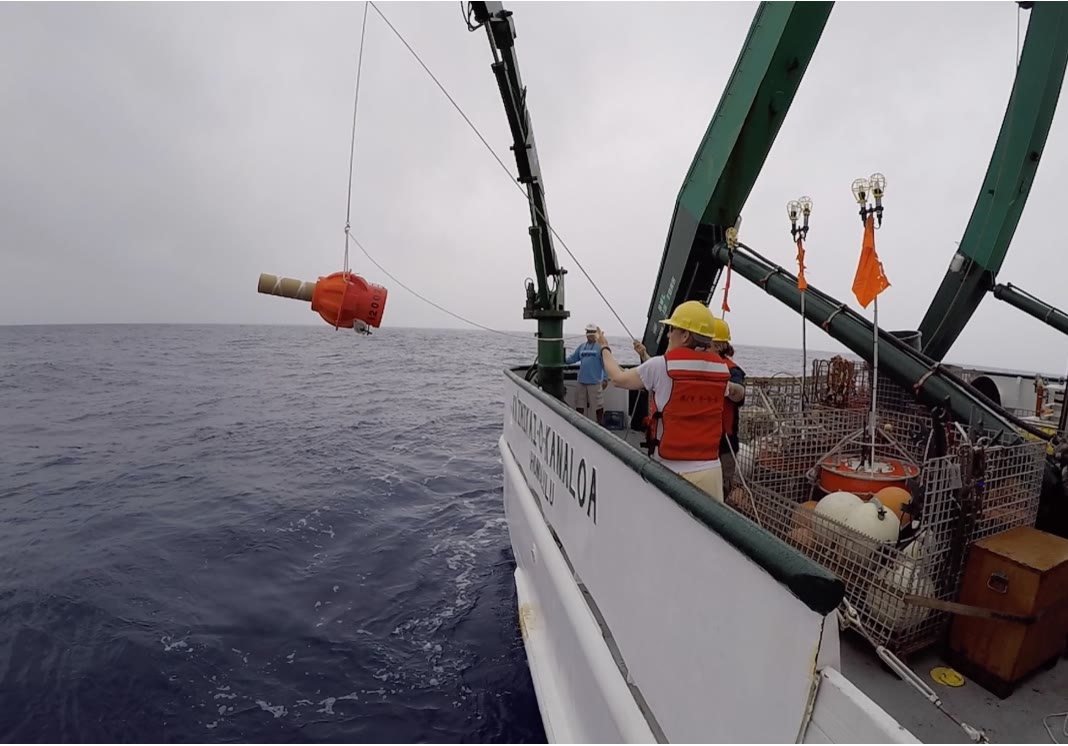
\includegraphics[width=0.6\linewidth]{images/book3/b1-deep-float.jpg}

{\small عوّامة قياس للمحيط العميق (الأداة البرتقالية المعلّقة بالرافعة) تُنزل من سفينة بحث في 2018؛ وبعد إطلاقها تغوص إلى عمق عملها، وتطفو على فترات منتظمة لإرسال بياناتها. (مصوّر مجهول من NOAA, ملك عام، عبر Wikimedia Commons.)}
\label{fig:b1:ocean-circulation:float}
\end{omfigure}
% ledger: commons:deep-solo, noaa:argo-25

ينقل الانقلاب الحرارة. فالماء الذي يتّجه شمالًا دافئًا ويعود باردًا قد أعطى حرارته للغلاف الجوي في الشمال.

\begin{proposition}[الحرارة التي يحملها الانقلاب]\label{prop:b1:ocean-circulation:heat}
إذا عبر تدفّق حجمي $Q$ خطّ عرض نحو الشمال عند درجة حرارة كامنة $\theta_1$ وعاد جنوبًا عند $\theta_2$، دون نقل صافٍ للكتلة، يحمل الانقلاب نحو الشمال تدفّق الحرارة
\[
  H = \rho c_p\,Q\,(\theta_1 - \theta_2),
\]
حيث $c_p$ الحرارة النوعية لماء البحر.
\end{proposition}
% ledger: teos10:cp0

\begin{proof}
في كل ثانية تعبر الكتلة $\rho Q$ نحو الشمال حاملةً محتوى الحرارة $\rho Q
c_p\theta_1$، مقاسًا من صفر تعسّفي للحرارة، وتعبر الكتلة نفسها جنوبًا حاملةً $\rho Q c_p\theta_2$. والتدفّق الصافي نحو الشمال هو الفرق؛ ولأن الكتلتين متساويتان، يلغي الصفر التعسّفي نفسه، والنتيجة نقل حقيقي للحرارة.
\end{proof}

حسب ميزانية تقديرية لشمال الأطلسي، لW.~Schmitz، يحمل تيّار الخليج \qty{40}{\sverdrup} من الماء عند \qty{18}{\celsius} شمالًا، منها \qty{14}{\sverdrup} تعود جنوبًا كماء عميق عند \qty{2}{\celsius}. ومع $c_p =
\qty{3992}{J.kg^{-1}.K^{-1}}$ و$\rho = \qty{1027}{kg.m^{-3}}$، يحمل هذا الانقلاب $1027 \times 3992 \times \num{14e6} \times 16 = \qty{0.92e15}{W}$، أي نحو \qty{0.9}{PW}، شمال \ang{24} شمالًا؛ والتقديرات الدقيقة تعطي \qty{1.2}{PW}، أي ربع نقل الحرارة نحو القطبين الذي يحمله الغلاف الجوي والمحيط معًا. ويُعطى معظم هذه الحرارة للهواء فوق شمال الأطلسي الشمالي، وهذا سبب واحد لكون النرويج، عند \ang{60} شمالًا، أدفأ بكثير من جنوب غرينلاند عند خطّ العرض نفسه.
% ledger: stewart:heat-conveyor, rapid:home, teos10:cp0 (computed in calc/ch29.py)

الدوران العميق بطيء. فإذا استغرق الماء الذي يغوص في شمال الأطلسي نحو ألف سنة ليصل المحيط الهادئ الشمالي عبر تيّار أنتاركتيكا الدائري، فإن متوسط سرعته نحو \qty{1}{mm/s}، أي أقلّ بمائة مرّة من التيّارات العميقة المتغيّرة التي يسجّلها مقياس التيّار. ولذلك تُستنتج سرعته من المتعقّبات لا تُقاس مباشرةً: فالتريتيوم، الذي أُطلق في الغلاف الجوي بتجارب الخمسينيات النووية ويتحلّل بنصف عمر 12.3 سنة، دخل الأطلسي الشمالي العميق حيث يتكوّن الماء العميق، وبعد 25 سنة امتدّ قليلًا جنوب \ang{30} شمالًا، أي متوسط سرعة أقلّ من \qty{1}{mm/s}. وحجم المحيط مقسومًا على معدّل تكوّن الماء العميق يعطي الرتبة الزمنية نفسها (\cref{exo:b1:ocean-circulation:12}).
% ledger: stewart:deep-circulation, nos:conveyor

يربط تيّار أنتاركتيكا الدائري الأحواض. تصل تياراته إلى قاع البحر وتكون بطيئة، نحو \qty{10}{cm/s}، وتبلغ \qty{50}{cm/s} عند جبهاته، لكنه عميق وعريض: فمصفوفة من مقاييس التيّار المرساة عبر مضيق دريك، بين أمريكا الجنوبية وأنتاركتيكا، أعطت \qty[uncertainty-mode=separate]{125 \pm
11}{\sverdrup} (نُشرت في 1985)، ومصفوفة أكثف في 2007--2011، قاست التيّارات قرب القاع أيضًا، أعطت \qty{173.3}{\sverdrup}، أي \qty{39}{\percent} أكثر من تلك القيمة المعتمدة منذ زمن طويل. وهو يحمل الماء العميق من كل محيط إلى الآخرين ويخلطه في الطريق.
% ledger: stewart:acc, donohue:acc

\begin{dated}{2021}
% ledger: ipcc:amoc-observed, ipcc:amoc-projected
يجد تقييم 2021 للهيئة الحكومية الدولية المعنية بتغيّر المناخ، من إعادات البناء، أن انقلاب الأطلسي كان مستقرًّا نسبيًّا على مدى ال\num{8000} سنة الماضية (\emph{ثقة متوسطة})، مع بداية ضعف في أواخر القرن التاسع عشر (\emph{ثقة متوسطة})، لكن لا تتوفّر إلا \emph{ثقة منخفضة} في وجود انحدار عام خلال القرن العشرين. والضعف المرصود مباشرةً من منتصف الألفينيات إلى منتصف العشرينيات (\emph{ثقة عالية}) لا يمكن تمييزه عن تقلّب بمقياس العقود (\emph{ثقة عالية}). ومن \emph{المرجّح جدًّا} أن يضعف الانقلاب خلال القرن الحادي والعشرين في كل سيناريوهات الانبعاث، مع \emph{ثقة منخفضة} فقط في حجم الانحدار؛ وهناك \emph{ثقة متوسطة} في أنه لن ينهار فجأة قبل 2100.
\end{dated}

\section{التمارين}

\begin{exercise}[$\star$]\label{exo:b1:ocean-circulation:1}
استخدم الصيغة الجمعية مع $\rho_a = \qty{1.3}{kg.m^{-3}}$ ومعامل السحب لYelland and Taylor. (أ)~احسب $C_D$ \omterm{def:b1:ocean-circulation:wind-stress}{وإجهاد الريح} لرياح قدرها \qty{4}{m/s}، و\qty{7}{m/s}، و
\qty{15}{m/s}. (ب)~بكم يتضاعف الإجهاد من \qty{7}{m/s} إلى \qty{15}{m/s}؟ قارن بنسبة مربّعي السرعتين واشرح الفرق.
% ledger: stewart:wind-stress, stewart:drag-coefficient
\end{exercise}

\begin{exercise}[$\star$]\label{exo:b1:ocean-circulation:2}
أعطِ اتجاه \omterm{def:b1:ocean-circulation:ekman}{نقل إيكمان} في كل حالة. (أ)~ريح تهبّ نحو الشرق عند \ang{45} شمالًا. (ب)~ريح تجارية من الشمال الشرقي عند \ang{15} شمالًا. (ج)~ريح تهبّ نحو الشرق عند \ang{50} جنوبًا. (د)~ريح من الجنوب على طول الساحل الغربي لجنوب أفريقيا، قرب \ang{23} جنوبًا. في أيّ الحالات الأربع يشير النقل نحو البحر، وماذا يترتّب على ذلك؟
\end{exercise}

\begin{exercise}[$\star$]\label{exo:b1:ocean-circulation:3}
عند \ang{26.5} شمالًا في الأطلسي، المتوسطات للفترة 2004--2024 هي: مضيق فلوريدا \qty{31.7}{\sverdrup}، \omterm{def:b1:ocean-circulation:ekman}{ونقل إيكمان} \qty{3.5}{\sverdrup}، والمحيط الأوسط العلوي \qty{-17.9}{\sverdrup}؛ وحسب الطبقات، 0--\qty{800}{m} \qty{16.6}{\sverdrup}، 800--\qty{1100}{m} \qty{0.4}{\sverdrup}، 1100--\qty{3000}{m} \qty{-12.0}{\sverdrup}، 3000--\qty{5000}{m} \qty{-5.9}{\sverdrup} (الاتجاه نحو الشمال موجب). (أ)~اجمع الثلاثة الأولى وقارنها بالانقلاب المنشور، \qty{17.1}{\sverdrup}. (ب)~قارن التدفّق نحو الشمال فوق \qty{1100}{m} بالتدفّق نحو الجنوب تحته. (ج)~حوّل \qty{17.1}{\sverdrup} إلى كيلومترات مكعّبة في السنة، واحسب الزمن الذي يستغرقه هذا التدفّق لملء حجم المحيط كله، \qty{1.3324e9}{km^3}.
% ledger: rapid:transports, charette:ocean-volume
\end{exercise}

\begin{exercise}[$\star$]\label{exo:b1:ocean-circulation:4}
بمعادلات إيكمان، احسب عمق إيكمان وتيّار السطح تحت ريح قدرها \qty{10}{m/s} عند \ang{15} و\ang{45} و\ang{60} من خطّ العرض، ونسبة تيّار السطح إلى الريح مئويًّا. لماذا تنهار الصيغ قرب خطّ الاستواء؟
% ledger: stewart:ekman-constants
\end{exercise}

\begin{exercise}[$\star\star$]\label{exo:b1:ocean-circulation:5}
عبر \ang{11} شمالًا في الأطلسي، خذ متوسط \omterm{def:b1:ocean-circulation:wind-stress}{إجهاد الريح} \qty{0.07}{Pa} نحو الغرب عبر عرض قدره \qty{5000}{km}، و$\rho = \qty{1027}{kg.m^{-3}}$. (أ)~احسب \omterm{def:b1:ocean-circulation:ekman}{نقل إيكمان} لكل متر واتجاهه. (ب)~احسب مجموع النقل الحجمي عبر المقطع بوحدة \omterm{def:b1:ocean-circulation:ekman}{السفيردروب}. (ج)~قارنه بالنقولات المقاسة مباشرةً ($12.0 \pm \qty{5.5}{\sverdrup}$) والمحسوبة من الرياح طويلة الأمد ($13.5 \pm \qty{0.3}{\sverdrup}$).
% ledger: stewart:ekman-transport
\end{exercise}

\begin{exercise}[$\star\star$]\label{exo:b1:ocean-circulation:6}
على طول المحيط الهادئ الاستوائي، تمارس \omterm{def:b1:atmospheric-circulation:winds}{الرياح التجارية} إجهادًا قدره \qty{0.05}{Pa} نحو الغرب. (أ)~احسب \omterm{def:b1:ocean-circulation:ekman}{نقل إيكمان} لكل متر، واتجاهه، عند \ang{2} شمالًا وعند \ang{2}~جنوبًا. (ب)~بافتراض أن الماء المحمول بعيدًا عبر هذين خطّي العرض يُستبدل من الأسفل بينهما، احسب متوسط سرعة \omterm{def:b1:ocean-circulation:upwelling}{الصعود} بالأمتار في اليوم. (ج)~ماذا يحدث لصيغة المبرهنة عند خطّ الاستواء نفسه؟ أيّ استنتاج يبقى؟
\end{exercise}

\begin{exercise}[$\star\star$]\label{exo:b1:ocean-circulation:7}
فوق دوّامة شبه مدارية، خذ إجهاد ريح \qty{0.06}{Pa} نحو الغرب عند \ang{15} شمالًا، و\qty{0.12}{Pa} نحو الشرق عند \ang{40} شمالًا. (أ)~احسب نقلي إيكمان واتجاهيهما. (ب)~بافتراض أن النقل يتغيّر بانتظام بين خطّي العرض، احسب السرعة الرأسية عند قاعدة \omterm{def:b1:ocean-circulation:ekman}{طبقة إيكمان}، بالأمتار في السنة، وقل هل هي صاعدة أم هابطة. (ج)~عبر حوض عرضه \qty{5000}{km}، كم \omterm{def:b1:ocean-circulation:ekman}{سفيردروب} يُضخّ عبر قاعدة الطبقة؟
\end{exercise}

\begin{exercise}[$\star\star$]\label{exo:b1:ocean-circulation:8}
خذ $\rho = \qty{1027}{kg.m^{-3}}$ و$c_p = \qty{3992}{J.kg^{-1}.K^{-1}}$. (أ)~احسب الحرارة المحمولة شمالًا بتدفّق قدره \qty{17}{\sverdrup} نحو الشمال عند \qty{15}{\celsius} يعود عند \qty{3}{\celsius}. (ب)~قارنها ب\qty{1.2}{PW} التي يحملها انقلاب الأطلسي. (ج)~لو عاد الماء نفسه جنوبًا عند السطح، على الجانب الشرقي للحوض، عند \qty{12}{\celsius}، ما الحرارة التي كان سيحملها؟ ماذا يقول هذا عن أهمية \omterm{def:b1:ocean-circulation:moc}{تكوّن ماء الأعماق}؟
% ledger: rapid:home, teos10:cp0
\end{exercise}

\begin{exercise}[$\star\star$]\label{exo:b1:ocean-circulation:9}
ثلاث كتل مياه في جنوب الأطلسي لها درجات حرارة كامنة وملوحات: ماء أنتاركتيكا المتوسط \qty{3.3}{\celsius}، 34.15؛ وماء الأطلسي الشمالي العميق \qty{4.0}{\celsius}، 35.00؛ وماء أنتاركتيكا القاعي \qty{0.4}{\celsius}، 34.67. عيّنة على عمق لها $\theta = \qty{2.78}{\celsius}$ و$S = 34.731$. باستخدام \cref{prop:b1:fluid-envelopes-structure:mixing}، أوجد كسر كل كتلة مياه في العيّنة.
% ledger: stewart:deep-circulation
\end{exercise}

\begin{exercise}[$\star\star\star$]\label{exo:b1:ocean-circulation:10}
خذ اللولب في \cref{prop:b1:ocean-circulation:spiral}. (أ)~بيّن أن $u$ و$v$ تحقّقان $f v + A_z u'' = 0$ و$-f u + A_z v'' = 0$. (تلميح: اكتب $u + iv =
V_0\,e^{i\pi/4}\,e^{(1+i)az}$.) (ب)~بيّن أن الإجهاد $\rho A_z\,\partial\vec
v/\partial z$ عند السطح يساوي \omterm{def:b1:ocean-circulation:wind-stress}{إجهاد الريح} $(0, T)$. (ج)~احسب النقلين $\int_{-\infty}^0 \rho u\,\mathrm dz$ و$\int_{-\infty}^0 \rho
v\,\mathrm dz$، وتحقّق من أنهما يتّفقان مع \cref{thm:b1:ocean-circulation:ekman}.
\end{exercise}

\begin{exercise}[$\star\star\star$]\label{exo:b1:ocean-circulation:11}
في نموذج ستوميل يبلغ عرض \omterm{def:b1:ocean-circulation:wbc}{تيّار الحدّ الغربي} نحو $R/\beta$، حيث $R$ معدّل احتكاك القاع، و$\beta = \mathrm df/\mathrm dy$ معدّل الزيادة نحو الشمال \omterm{def:b1:atmospheric-circulation:coriolis-parameter}{لمعامل كوريوليس}. (أ)~بيّن أن $\beta = 2\Omega
\cos\varphi/a_\oplus$ واحسبه عند \ang{30} شمالًا ($a_\oplus = \qty{6371}{km}$). (ب)~مع $R = \qty{e-6}{s^{-1}}$، احسب العرض. (ج)~ينجرف نقل قدره \qty{30}{\sverdrup} نحو الجنوب عبر داخل حوض عرضه \qty{5000}{km} في الألف متر العليا، ويعود شمالًا في تيّار الحدّ عبر العمق نفسه. احسب السرعتين المتوسطتين وقارنهما بسرعة تيّار الخليج، \qty{1.8}{m/s}.
% ledger: stewart:north-atlantic, nos:gulf-stream, earth:Rmean
\end{exercise}

\begin{exercise}[$\star\star\star$]\label{exo:b1:ocean-circulation:12}
يحتوي المحيط على \qty{1.3324e9}{km^3} فوق \qty{361.84e6}{km^2}. (أ)~بيّن أن الحجم تحت \qty{1000}{m} لا يقل عن \qty{9.71e8}{km^3}. (ب)~يتكوّن الماء العميق لشمال الأطلسي بنحو \qty{17}{\sverdrup}، وماء أنتاركتيكا القاعي بنحو \qty{9}{\sverdrup}. قدّر الزمن اللازم لتجديد الماء تحت \qty{1000}{m}، وقارنه بالألف سنة للناقل. (ج)~نصف عمر التريتيوم 12.3 سنة. ما الكسر من مدخل تريتيوم يبقى بعد 25 سنة؟ إلى أيّ مسافة يقطع ماء يتحرّك بسرعة \qty{1}{mm/s} في 25 سنة؟
% ledger: charette:ocean-volume, stewart:deep-circulation, stewart:acc, rapid:transports
\end{exercise}

\section{مسألة: ساحل ذو صعود}

\begin{problem}[{مسألة نهاية الأسبوع --- ريح صيفية على ساحل عند \ang{38} شمالًا}]
\label{pb:b1:ocean-circulation:1}
% values: calc/ch29.py (invented coast; constants from the ledger)
يمتدّ ساحل مستقيم شمال–جنوب عند \ang{38} شمالًا، والمحيط إلى الغرب. وفي الصيف تهبّ ريح ثابتة قدرها \qty{8}{m/s} من الشمال على طوله لأسابيع. الساحل مخترَع، لكن أرقامه نموذجية للجوانب الشرقية للمحيطات. استخدم $\Omega = 2\pi/(\qty{23.9345}{h})$، و$\rho_a = \qty{1.3}{kg.m^{-3}}$، ومعامل السحب لYelland and Taylor، و$\rho = \qty{1027}{kg.m^{-3}}$ لماء البحر، و$c_p = \qty{3992}{J.kg^{-1}.K^{-1}}$.

\medskip
\noindent\textbf{الجزء الأول --- الريح وإجهادها.}
\begin{enumerate}
  \item نحو أيّ اتجاه تهبّ الريح؟ هل هي على طول الساحل أم عبره؟
  \item احسب معامل السحب.
  \item احسب \omterm{def:b1:ocean-circulation:wind-stress}{إجهاد الريح}.
  \item السؤالان نفسهما لريح قدرها \qty{12}{m/s}. بكم يزداد الإجهاد، ولماذا يزيد على نسبة مربّعي السرعتين؟
  \item احسب \omterm{def:b1:atmospheric-circulation:coriolis-parameter}{معامل كوريوليس} عند \ang{38} شمالًا.
  \item احسب $2\pi/f$ بالساعات. لماذا يجب أن تهبّ الريح يومًا أو أكثر قبل أن ينطبق توازن إيكمان؟
\end{enumerate}

\medskip
\noindent\textbf{الجزء الثاني --- \omterm{def:b1:ocean-circulation:ekman}{طبقة إيكمان}.}
\begin{enumerate}[resume]
  \item في أيّ اتجاه يجري \omterm{def:b1:ocean-circulation:ekman}{نقل إيكمان}؟ نحو اليابسة أم البحر المفتوح؟
  \item احسب كتلة \omterm{def:b1:ocean-circulation:ekman}{نقل إيكمان} لكل متر من الساحل.
  \item حوّلها إلى نقل حجمي لكل متر.
  \item احسب عمق إيكمان بصيغة إيكمان.
  \item احسب متوسط السرعة نحو البحر في الطبقة، بوحدة \unit{cm/s}.
  \item احسب تيّار السطح بصيغة إيكمان واتجاهه. ماذا تقترح قياسات العوّامات عن سرعته بدلًا من ذلك؟
\end{enumerate}

\medskip
\noindent\textbf{الجزء الثالث --- \omterm{def:b1:ocean-circulation:upwelling}{الصعود} عند الساحل.}
\begin{enumerate}[resume]
  \item فسّر، برسم تخطيطي لمقطع رأسي، من أين يأتي الماء المحمول بعيدًا.
  \item احسب حجم الماء المصعَّد في اليوم على طول كل كيلومتر من الساحل.
  \item افترض أن الماء يرتفع عبر شريط عرضه \qty{20}{km} على طول الساحل. احسب متوسط السرعة الرأسية الصاعدة، بوحدة \unit{m/s} وبالأمتار في اليوم.
  \item كم يستغرق الماء ليرتفع من قاعدة \omterm{def:b1:ocean-circulation:ekman}{طبقة إيكمان} إلى السطح بهذه السرعة؟
  \item يصل الماء المصعَّد إلى السطح عند \qty{12}{\celsius}، بينما البحر المفتوح قبالته عند \qty{18}{\celsius}. يحمل نسيم البحر هواءً دافئًا رطبًا من البحر المفتوح فوق هذا الماء. ماذا يحدث للهواء قرب السطح، وأيّ طقس يتبع ذلك على الساحل؟
  \item لماذا تكون هذه السواحل غنية بالسمك؟
  \item في الخريف تتحوّل الريح وتهبّ من الجنوب أسبوعًا. ماذا يحدث للنقل وللماء عند الساحل؟
\end{enumerate}

\medskip
\noindent\textbf{الجزء الرابع --- سواحل أخرى والنقل الكلّي.}
\begin{enumerate}[resume]
  \item بالإجهاد نفسه، احسب \omterm{def:b1:ocean-circulation:ekman}{نقل إيكمان} لكل متر عند \ang{20} شمالًا، وقارنه ب\ang{38} شمالًا.
  \item على الساحل الغربي لجنوب أفريقيا، قرب \ang{23} جنوبًا، أيّ اتجاه للريح يقود \omterm{def:b1:ocean-circulation:upwelling}{الصعود}؟ قارنه بساحل المسألة.
  \item تحت ريح قدرها \qty{5}{m/s} بدلًا من \qty{8}{m/s} عند \ang{38} شمالًا، احسب الإجهاد \omterm{def:b1:ocean-circulation:ekman}{ونقل إيكمان} لكل متر، ونسبتهما إلى تلك الخاصة بالسؤال~8.
  \item يُسخَّن الماء المصعَّد بمقدار \qty{6}{\celsius} وهو ينجرف نحو البحر. احسب الحرارة التي يمتصّها في الثانية لكل متر من الساحل، ثم على طول \qty{1000}{km}.
  \item ما طول ساحل كهذا يُصعِد الماء بقدر ما يحمله تيّار الخليج عبر مضيق فلوريدا، \qty{31.7}{\sverdrup}؟
  \item ما حجم الماء، \omterm{def:b1:ocean-circulation:ekman}{بالسفيردروب}، الذي يُصعَد على طول \qty{1000}{km} من هذا الساحل؟
\end{enumerate}
\end{problem}
